\documentclass[10pt]{beamer}
\usepackage[utf8]{inputenc}
\usepackage[T1]{fontenc}
\newif\ifpt
\usepackage{user}
\ifpt
\usepackage[portuguese]{babel}
\else
\usepackage[english]{babel}
\fi
\usepackage{graphicx}
\usepackage{color}

\colorlet{mybasecolor}[rgb]{blue!60!black}
\usepackage{slidesdef}

\author{\autor}
\title{\titulo}
\date{\data}

\begin{document}

\myframe{
  \begin{beamercolorbox}[center, rounded=true, shadow=true]{mainbox}
    \bf \LARGE \titulo
  \end{beamercolorbox}
  \hfill
  \begin{beamercolorbox}[center, wd=0.8\textwidth, rounded=true,
      shadow=true]{secbox}
    \bf \large \evento
  \end{beamercolorbox}
  \hfill{}

  \linespread{1.0}
  \begin{center}
    \textbf{\autor}
    \vspace{-4pt}
    {\scriptsize \\ \instautor}
    \ifdefined\colabum
      \vspace{10pt}
      \textbf{\\ \colabum}
      \vspace{-4pt}
      {\scriptsize \\ \instcolabum}
    \fi
    \ifdefined\colabdois
      \vspace{10pt}
      \textbf{\\ \colabdois}
      \vspace{-4pt}
      {\scriptsize \\ \instcolabdois}
    \fi
    \ifdefined\colabtres
      \vspace{10pt}
      \textbf{\\ \colabtres}
      \vspace{-4pt}
      {\scriptsize \\ \instcolabtres}
    \fi
    \ifdefined\colabquatro
      \vspace{10pt}
      \textbf{\\ \colabquatro}
      \vspace{-4pt}
      {\scriptsize \\ \instcolabquatro}
    \fi
    {\small \\ \vfill \data}
  \end{center}
}

\myframe{
  \ctr{Bem Vindos}
  \ctr{Estamos atrasados}
}

\myframe{
  \ctr{Estamos atrasados}
  \begin{itemize}
    \item A computação não é limitada por artigos;
    \item Internet, celulares, tablets, relógios\ldots;
    \item ``O matemático aplicado que tem que fazer a ponte'';
    \item Colaborações à distância.
  \end{itemize}
}

\myframe{
  \ctr{Todo mundo deveria aprender programação}
  \begin{itemize}
    \item ``I think everybody in this country should learn how to program a
      computer because it teaches you how to think.'' - Jobs, S.;
    \item Desenvolvimento de lógica e \emph{problem-solving skills};
    \item Facilitar algumas tarefas;
    \item Entender o mundo.
  \end{itemize}
}

\myframe{
  \ctr{Todo matemático deveria aprender programação}
  \begin{itemize}
    \item Melhorar a aula;
    \item Testar a teoria;
    \item Colaborar com outras pessoas.
  \end{itemize}
}

\myframe{
  \ctr{Terminal - Bash}
  \begin{itemize}
    \item Começamos aqui;
    \item Algumas coisas não se fazem com mouse;
    \item Grande quantidade de ferramentas;
    \item Todo computador (GNU/Linux) tem.
  \end{itemize}
}

\myframe{
  \ctr{Julia}
  \begin{itemize}
    \item Uma boa linguagem para pesquisadores das ciências exatas;
    \item Uma boa linguagem inicial;
    \item Almeja substituir o MatLab;
    \item Usa coisas boas de outras linguagens (C, Fortran, MatLab,
      Python,\ldots);
    \item Código aberto, ativamente desenvolvida.
  \end{itemize}
}

\myframe{
  \ctr{Git}
  \begin{itemize}
    \item Principal ferramenta livre de controle de versão;
    \item Colaboração;
    \item Qualquer arquivo de texto binário (\LaTeX, códigos);
    \item Versões diferentes (versão estável, de debug, conserto, nightly,
      etc.);
    \item Interfaces web e local para repositórios públicos e privados.
  \end{itemize}
}

\myframe{
  \begin{center}
    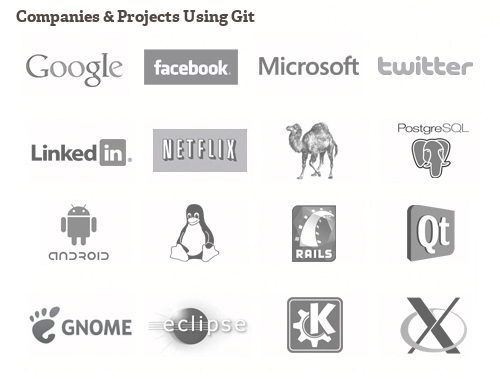
\includegraphics[height=0.9\textheight]{img/using-git.png}
  \end{center}
}


\myframe{
  \hfill
  \begin{beamercolorbox}[center, wd=0.6\textwidth, rounded=true,
      shadow=true]{secbox}
    \bf \LARGE \thanksmsg
  \end{beamercolorbox}
  \hfill{}

  \begin{center}
    \includegraphics[scale=0.7]{img/cc.png} \qquad
    \includegraphics[scale=0.7]{img/by.png} \qquad
    \includegraphics[scale=0.7]{img/sa.png}

  \ifpt{
    Esta apresentação está licenciada com uma Licença Creative Commons
    Atribuição-CompartilhaIgual 4.0 Internacional.
  }\else{
    This presentation is licensed under the Creative Commons Attributions-ShareAlike 4.0
    International License.
  }\fi
  \end{center}
}

\end{document}
